\documentclass[sigconf,natbib=false, language=english]{acmart}

% Ne dodajaj hyperref (acmart ga že naloži)
\settopmatter{printccs=false, printacmref=false}


% BEGIN BIBLIOGRAPHY CONFIGURATION
% --------------------------------------------- %

\usepackage[datamodel=acmdatamodel, style=acmnumeric, backend=biber]{biblatex}
\addbibresource{refs.bib}
\renewcommand*{\bibfont}{\small}

% --------------------------------------------- %
% END BIBLIOGRAPHY CONFIGURATION

\AtBeginDocument{%
  \providecommand\BibTeX{{%
    Bib\TeX}}}

\setcopyright{rightsretained}
\copyrightyear{2025}
\acmDOI{}
\acmISBN{}
\acmConference[Information Society 2025]{Information Society 2025: 28th international multiconference}{6--10 October 2025}{Ljubljana, Slovenia}
\settopmatter{printccs=false, printacmref=false}

\geometry{a4paper}
\begin{document}


\title[Ski Jumping Simulation]{Predicting ski jumps using state-space model}


\author{Živa Hegler}
\affiliation{%
  \institution{Univerza v Ljubljani}
  \city{Ljubljana}\country{Slovenia}}


\author{Neca Camlek}
\affiliation{%
  \institution{Univerza v Ljubljani}
  \city{Ljubljana}\country{Slovenia}}

\author{Marko Grobelnik}
\affiliation{%
  \institution{Jožef Stefan Institute}
  \city{Ljubljana}\country{Slovenia}}
\email{marko.grobelnik@ijs.si}

\renewcommand{\shortauthors}{Ž. Hegler and N. Camlek}


\begin{abstract}

Ski jumping performance is shaped by both athlete technique and environmental 
conditions, with factors such as wind speed, wind direction, and ski orientation 
playing a critical role in determining jump trajectories. Accurate modeling of 
these trajectories is challenging due to the system’s dynamic and time-dependent\\ 
nature. In this work, we introduce a dataset of measured ski jumps and present a 
state-space modeling framework that captures the evolution of jumps under varying 
conditions. The model parameters are estimated using a ridge regression approach, 
enabling us to predict trajectories from initial states and wind sensor inputs. 
We evaluate the predictive performance of the model through leave-one-out cross-validation 
and analyze its stability, showing that the approach can generate realistic trajectories 
with reasonable accuracy. To complement the modeling results, we developed an interactive 
web application that allows users to \\
explore both recorded and simulated jumps, adjust 
environmental factors, and visualize their effects through animations. Together, the 
dataset, modeling framework, and application offer a foundation for further research in 
ski jump analysis and provide an accessible tool for exploring the influence of external 
conditions on performance.

\end{abstract}

\keywords{datasets, SSM, ski jumping, simulations, least squares}

%%\received{20 August 2025}
%%\received[revised]{13 September 2025}
%%\received[accepted]{15 September 2025}

%% This command processes the author and affiliation and title
%% information and builds the first part of the formatted document.
\maketitle

\section{Introduction}
%kaj delava
%kaj je problem in kako ga drugi rešujejo
%piševa na kakšne načine drugi lahko to delajo, kakšne opcije obstajajo


Ski jumping is a sport strongly influenced by both athletic \\
technique and environmental conditions.
Factors such as wind speed, wind direction, and different ski angles affect the trajectory 
and final distance of a jump, making accurate prediction a challenging problem. 
While statistical models and simulations have been applied in sports research for 
some time, many approaches\\ simplify the problem and do not fully capture the dynamic 
evolution of the jump over time.

Recent advances in machine learning have introduced methods capable of modeling 
temporal systems with greater fidelity. In particular, state space models provide 
a mathematical framework for representing hidden internal states that evolve over time 
in response to external inputs. This makes them well-suited for modeling ski jumps, 
where environmental factors determine performance.

In this paper, we present a dataset of ski jumps together with a state space model 
trained to predict jump trajectories based on changing environmental conditions. 
The model is estimated using a least squares approach and demonstrates how inputs 
such as wind and ramp adjustments influence the resulting jump. Beyond the modeling 
framework, we also developed an application that allows general users to interact with 
the data, run simulations, and visualize jump trajectories through animations. 

The remainder of the paper is as follows. Section~\ref{sec:data} presents the handling 
of received data. Next, the proposed methodology is described in Section~\ref{sec:method}. 
The project results are presented in Section~\ref{sec:results}. We discuss the results in 
Section~\ref{sec:discussion} and conclude the paper in Section~\ref{sec:conclusion}.

%%okej zdi se mi, da nimava za govort o nobenem related work, ker ne vem ce obstaja kej 
tazga oz ni neka ful razsirjena zadeva, zato se ta odstavek zdej imenuje Data

\section{Modeling Framework and Dataset}\label{sec:data}
This section describes the data handling, focusing on state space models and our 
data processing.

\subsection{State Space Model}\label{subsec:ssm}
State Space Models (SSMs \cite{aoki1990state}) are a family of machine learning algorithms designed to 
capture and predict the behavior of dynamic systems by describing how their inner 
state changes over time. 
Instead of only looking at past inputs and outputs, SSMs explicitly model the 
underlying dynamics, making them well-suited for sequential data. In state space modeling, 
the objective is to identify the minimal set of system variables required to completely 
describe the system. These fundamental variables are referred to as the state variables. 
At any given time, the state of the system can be represented by a state vector, 
whose components correspond to the values of the respective state variables. 
SSMs are designed to predict both the manner in which inputs are reflected in the 
system's outputs and the evolution of a system's internal state over time and in 
response to specific inputs. \cite{SSM_YouTube}

\subsection{Least squares method}

The least squares method (LS \cite{Plestenjak_NUM}) is a regression technique that is used to 
determine the line that best fits a given set of data. It minimizes the sum 
of the squared differences between the observed data and the corresponding 
values implied by the regression function. Each data point reflects the relationship 
between a known independent variable and an unknown dependent variable.

To enhance the model, we incorporated ridge regression (L2 regularization), which 
helps reduce overfitting during model training. \cite{vanWieringen2015ridge}

\subsection{Data Processing}

%vse o podatkih: kakšne podatke sva dobili in kje sva jih dobili, kaj je blo v njih, 
%kako jih je blo treba spremenit lahko tko po korakih kaj je blo treba spreminjat, 
%da so bli za uporabo, lahko tko po korakih: naprej je blo treba to in pol to...

For our project we used 223 CSV files, each containing the data of one jump. 
Each contains 17 columns ('Position', 'Height above ground', 'Time', 'X', 'Y', 'Z', 
'Opening Angle', 'Stalling Angle Left', 'Stalling Angle Right', 
'Roll Angle Left', 'Roll Angle Right', 'Yaw Angle Left', 'Yaw Angle Right', 
'Speed hor.', 'Speed vert.', 'Speed resulting', 
'WindTime|WindName|WindSpeed|Wind...')
and number of rows corresponding to the length of the jump. Data is recorded for every meter
of air distance from the take-off point. of air distance from the take-off point.

The data required some pre-processing before it could be used for training the model.
The column Time was written using the format: $0001-01-01\text{T}00:00:00.0000000+01:00$. Here, 
$0001-01-01$ means the date (January first in the year one), which is a place holder date, so we removed it.
The $+01:00$ at the end indicates the time zone, which we also removed.
The remaining part $00:00:00.0000000$ indicates the time of the jump in hours, minutes, seconds and milliseconds.
We converted this to a numerical value in seconds, which was then used as the time variable in the model.
The column 'WindTime|WindName|WindSpeed|Wind...' contained multiple pieces of information separated by '|'.
The wind was recorded on 12 sensors placed along the hill, each measuring one of the seven wind feature in the order 
represented in the column name. To keep all the data and not multiply the time stamps, we split this 
column into $12 \cdot 6 = 72$ columns, each representing one of the wind features for one of the sensors (\texttt{sensor\_feature}).

%I THINK DA BI BLO DOBR DA TUD ZA KOTE DODAVA NEKO SLIKO
\begin{description}
    \item[Position] - air distance from the take-off point in meters. Begins with a negative value, which
    represents the distance from the starting point to the take-off point. In ski jumping, the starting point
    is adjusted according to the wind conditions, so this value is not constant.
    \item[Height above ground] - height above the ground in meters.
    \item[Time] - time of the jump in seconds from the start of the jump.
    \item[X, Y, Z] - coordinates of the jumper in a 3D space in meters. The X axis is aligned with the hill direction,
    the Y axis is across the hill, and the Z axis is vertical. The take-off point is (0,0,0) as shown in figure~\ref{fig:planica}
    \item[Opening Angle] - angle between the skis in degrees.
    \item[Stalling Angle Left, Stalling Angle Right] - angle \\
    between the left/right ski and the horizontal plane in degrees.
    \item[Roll Angle Left, Roll Angle Right] - angle between the \\ left/right ski and the horizontal plane in degrees.
    \item[Yaw Angle Left, Yaw Angle Right] - angle between the \\ 
    left/right ski and the horizontal plane in degrees.
    \item[Speed hor., Speed vert., Speed resulting] - horizontal,\\
    vertical, and the resulting speed of the athlete in km/h.
\end{description}

\begin{figure}[h]
  \centering
  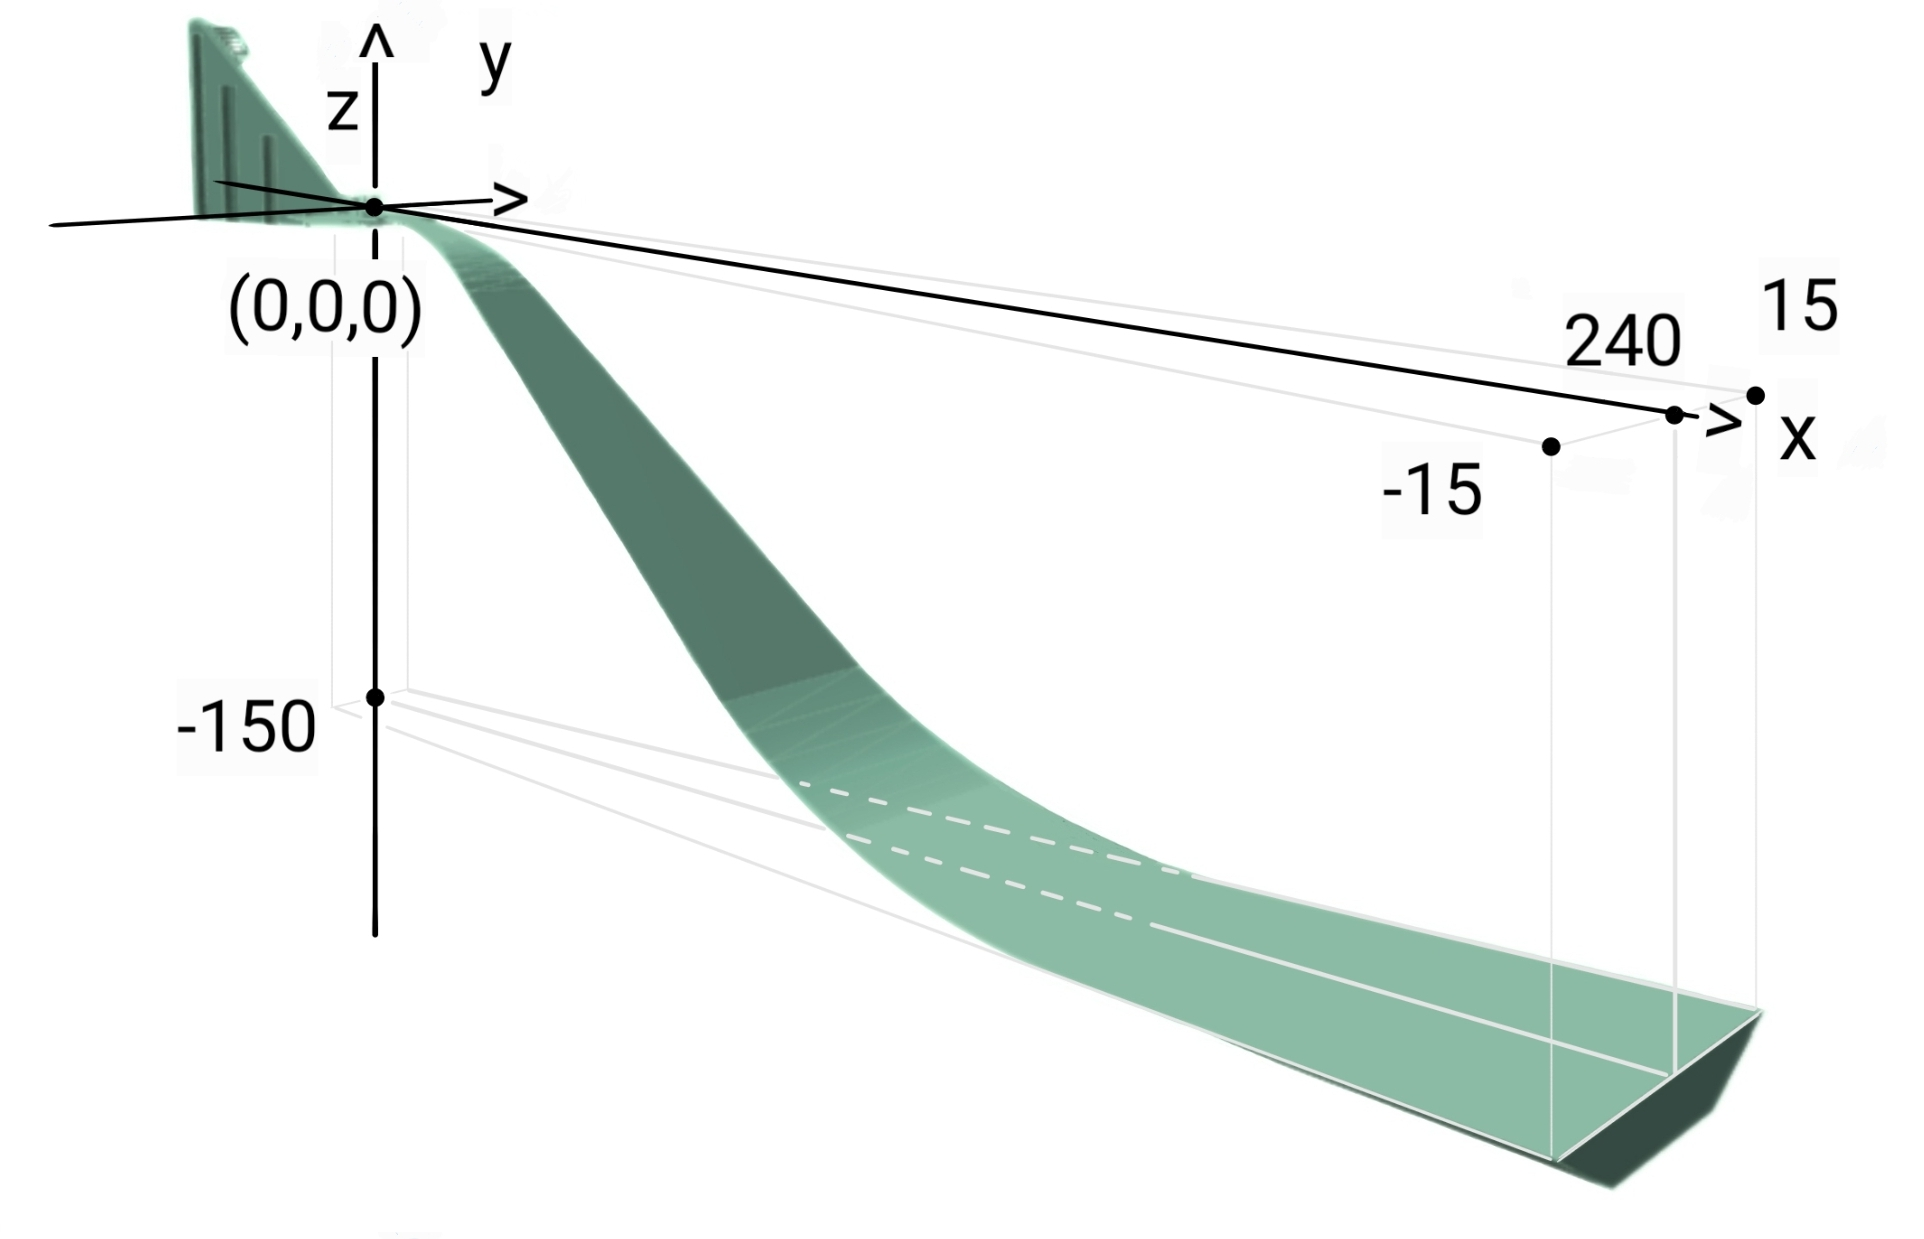
\includegraphics[width=\linewidth]{koncen_graf.jpg}
  \caption{3D model of Ski jump in Planica with added coordinates \cite{skisprungschanzen_letalnica} \cite{3dmdb_skijumping_planica}}
  \Description{A model of ski jump in Planica, showing X, Y and Z axis}
  \label{fig:planica}
\end{figure}

The wind features are as follows:
\begin{description}
    \item [WindTime] - time of the wind measurement in the same format as the Time column itself. Since wind measurements
    are recorded less often, the wind values are applied to the most recent jump measurement and then just \\
    repeated until a new wind measurement is available. Since the wind is represented by a nonlinear function, it would be hard to capture
    it's movements with interpolation, so we decided to drop this column.
    \item [WindName] - name of the sensor ( Wi for i = 1,...,12)
    \item [WindSpeed] - resulting speed of the wind in km/h 
    \item [WindSpeedTangent] - speed of the wind tangent measured along the x axis (hill direction) in km/h
    \item [WindTurbulence] - vertical speed of the wind turbulence in km/h
    \item [WindSpeedCleanTan] - wind speed tangent with\\
     turbulence removed in km/h
    \item [WindSpeedCross] - speed of the wind measurement along the y axis across the hill in km/h
\end{description}

There are 12 wind sensors spread across on the ski jumping hill. To help with
the analysis we separated the jumping section of the hill into 3 zones. The first zone
contains wind sensors 1 to 4, the second zone contains sensors 5 to 8 and the third zone
contains sensors 9 to 12.

During processing, we also removed some ski jumps that were incomplete or had corrupted data, so the
final data set contained around 200 ski jumps \cite{SkiJumping_Book}.

\section{Methodology}\label{sec:method}
This section outlines our research methodology. We first present different variations 
of the SSM that we tested for the ski jump simulation, followed by describing our model 
and how it predicts the jumps. Finally, we present the description of our ski jump 
animation app.

\subsection{Alternative modeling approaches}

%pač to je tko idejno, recimo k si probala različne stvari, kaj kako dela, sej 
%ne vem če sm prou napisala, če nism lahko popraviš, sam tko se je slišal fensi
%no tuki se mi zdi da na kratko sam kaj je blo probano polpa natancno kar mava 
%zdej v naslednjem subsectionu

Some of the alternative approaches we considered for modeling ski jumps included classical
physics-based models, but the data  isn't sufficient to accurately capture all the forces acting on the jumper.
We also tried a hybrid approach combining SSM and Physics-informed Neural Networks (PINNs \cite{Cai2021_PINN_FluidMechanics} \cite{StatQuest_NN_YouTube}), where
the SSM would provide a baseline prediction, and the PINN would learn to correct any discrepancies, where it takes into
account physical properties of the system, such as the mass of the pilot, wind properties and gravitational force. 
These parameters are included in the equations of motion, which are added to the overall loss function. 
So the model prefers solutions that are consistent with the laws of physics.. This
turned out to be less effective than a pure SSM approach. But the reason exceeds the this papers' purpose.


\subsection{Ski jump prediction model}

In order to fit our data to the SSM, we stored the data in for each file in three vectors.
The main vector contains states or state variables of the system, which in our case are the
X, Y and Z coordinates and velocitys of the jumper, and all the angles (opening, stalling, roll and yaw) \cite{CERN_SkiJump_Physics}.

The observation vector contains the measured outputs of the system, which in our case are the X, Y and Z coordinates
and height above ground. And the controls contain the external inputs to the system, which in our case are
the wind measurements from all the sensors, that are averaged over each zone and feature (speed, tangent, cross and turbulence).

We then used the ridge regression to estimate the matrices A, B, C and D of the SSM, where we minimize the computed values from current
and previous values and the next time stamp values.Thus the matrix A computes the next state from the current state, 
B computes the next state from the current control, C computes the next observation from the current state and D computes 
the next observation from the current control. We then use recursion to predict the next state from the prediction of the 
previous state and the current control, to get the full simulated jump. This allows us to predict the jump trajectory 
based on the environmental conditions and the starting state of the jumper.



\subsection{Ski jump animation app}

To make our results accessible beyond the research setting, we developed an 
interactive web application using Shiny for Python \cite{shiny_python}. The application serves as a 
front-end to the trained state space model and allows users to explore ski jump 
simulations under varying environmental conditions or just to observe different 
measured ski jumps. Through a set of input controls, users can adjust factors such 
as wind speed, wind directions, or different ski angles, and the application instantly 
updates the predicted jump trajectory.

The application presents the results as an animated visualization of the ski jump, 
showing the full trajectory and the final distance. In this way, the application 
functions both as an analytical tool, helping to test how different conditions affect 
performance, and as an educational resource that makes the mechanics of ski jumping 
more easier to understand for a wider audience.

\section{Main results}\label{sec:results}
In this section, we present the results of our simulations. Firstly, we present a 
statistical comparison of all the models, followed by a precise analysis of our 
predictions.

%kokr rezultati, kaj sva dosegli ig
%natančno opiševa kako sva preverjali kok dober je najin model in pač tudi poveva 
%kok dobr je najin model, mal še s tistimi napakami vrjetn pa tko

\subsection{Models' error}

In order to evaluate different models, we first had to define a metric for measuring the prediction error.
Since the actual and simulated jumps are represented with x, y, z coordinates, but are measured at different time stamps,
and can contain a different number of measurements, we had to find a way to compare them. We first tried to project
the shorter trajectory on to the other one and compute the distance between the the original and the projection, 
but this method turned out to be computationally expensive. So we later decided to compute the distance between 
the actual and the simulated jump by interpolating both jumps. The new measurements contain the start and the end point
and all the ones, where x reaches a natural value. We then compute the error as the norm of the difference between the two jumps.
And after one of the jumps ends, we just add the distance from the end of the shorter jump to the end of the longer jump
to the error. This way we penalize the model for not being able to predict the correct length of the jump.

Since we had a limited number of jumps, we used leave-one-out cross-validation to evaluate the models.
For each jump, we trained the model on all the other jumps and then simulated the left out jump. We then computed 
the average error between the actual and the simulated jump for both the training and the test set.

In the process of developing our ski jump prediction model, we evaluated several 
variations to determine the most effective approach. We compared the performance 
of a pure State Space Model (SSM) against a hybrid model that combined SSM with 
Physics-informed Neural Networks (PINNs). The pure SSM demonstrated superior predictive 
accuracy, likely due to its ability to directly model the temporal dynamics of ski jumps 
without the added complexity of PINNs.
We also experimented with different configurations of the SSM, including using
all available wind sensor data versus an averaged value of the zone. When we used all the sensors,
the average error for each point (on training data is 1.67m and on test data is 1.89m), while when we averaged the sensors 
over the zones the error (on training data was 1.76m and on test data 1.82m). This suggests that averaging the wind data helps
with the simulation.

\begin{figure}[h]
  \centering
  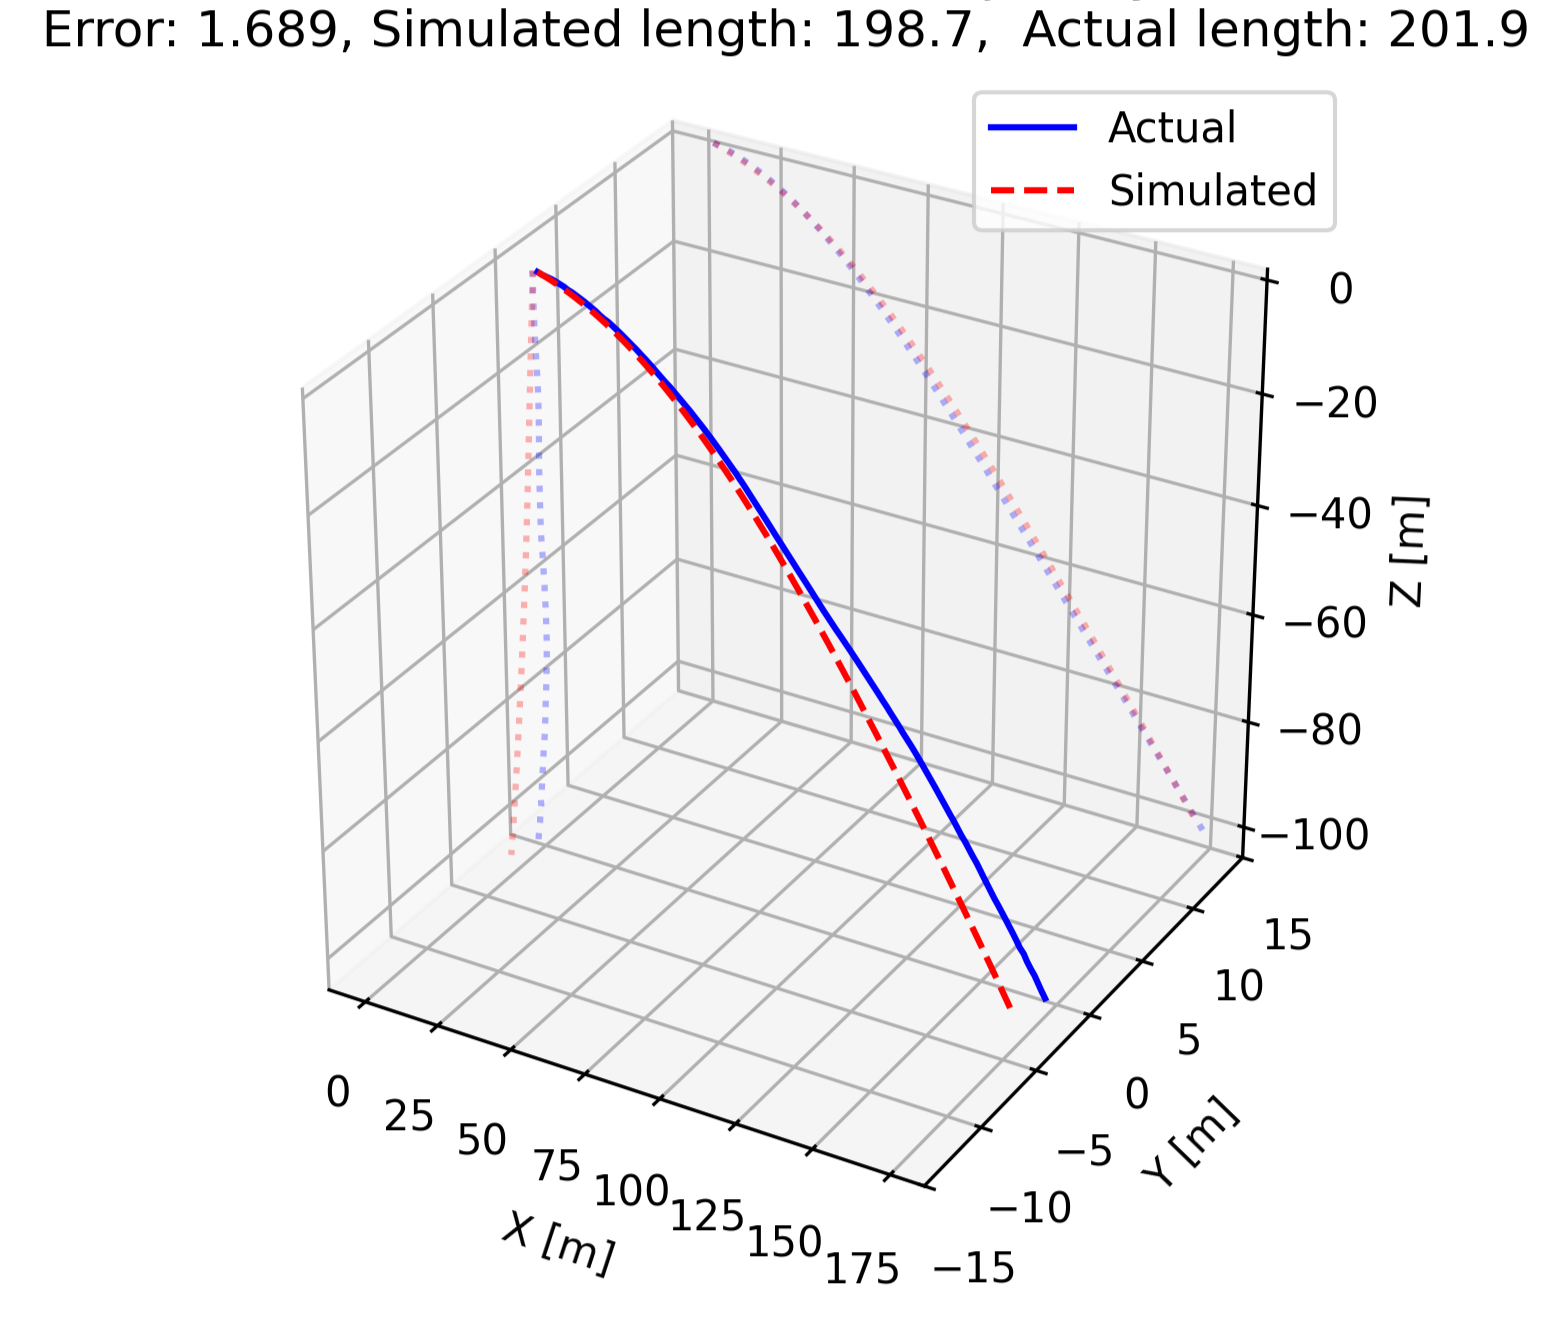
\includegraphics[width=\linewidth]{2SSM flight_simulation167-small.png}
  \caption{Actual vs. simulated ski jump trajectory}
  \Description{A graph comparing an actual jump trajectory to the simulated one}
  \label{fig:graph1}
\end{figure}

\subsection{Analysis of our model}

Since the wind is a very important factor in ski jumping, we also tried to capture 
the nonlinear movements of the wind by adding columns containing the square of the wind features.


Since the simulation still requires quite a few inputs, we also made the simulation
interactive, so the user can adjust the wind and see how it affects the jump.
On the ski jumping app the user can use sliders to choose the wind speed, wind tangent,
wind cross and wind turbulence for each of the three zones. This also means that the wind looses 
the actual movement function. The rest of the inputs are set to the average values 
of all the jumps in the dataset. 

%Because the predictions of the model are not perfect, we analyzed the errors in more detail.
%We first computed the error for each point of the jump and then averaged it over all the jumps.
%The error is the smallest at the beginning of the ju

\section{Discussion}
\label{sec:discussion}

%mal razglabljas o vsem, torej mal povežeš skupi kar sva do zdej povedali in 
%predlagava kkšne možne izboljšave mogoče
%torej najprej kok dobr je najna stvar delala, kako sva bli omejeni (mogoče da nisva meli ful velik podatkov?) in kaj še lahko in bova izboljsali


This section examines the predictive performance of the trajectories, highlights the 
limitations of our current approach, and suggests directions for future improvements.

\subsection{Limitations}

The main limitation of our project is the relatively small number of ski jumps 
available for training the model. After preprocessing, the dataset contained 
only about $200$ jumps, which may limit the SSM's ability to represent the full 
range of trajectory variations under different circumstances. As a result, the 
model may struggle to accurately predict jumps under novel or extreme conditions.

Additionally, the dataset lacks detailed information, or any information at all 
about individual jumpers, such as body weight, sex, or other physiological characteristics 
that are known to influence jump performance. Incorporating these variables 
could improve model accuracy and provide more personalized predictions.

Lastly, due to limited computing power, only one CPU with - of space was 
available, restricting the use of possible better models. To address these 
challenges, using cloud-based resources could help run larger models and 
improve the prediction of trajectories.

\subsection{Future work and potential improvements}

While the current approach shows promise, there are several avenues for future
improvements. Some of which we are working on as of the time of writing this paper.

currently we are working on improving the sliders functions. Since the wind data 
determined by the user is static throughout the jump this adds a lot of generalization.
In reality, wind conditions can change rapidly during a jump. So we would like to
add additional controls to the app that would allow the user to define how the wind changes
during the jump. They could choose whether the wind would be gaining or losing a certain feature
(such as speed or turbulence) during the jump.

Expanding the dataset to include more jumps and additional contextual 
information about individual jumpers could enhance model accuracy. We could
try to generate more data by using data augmentation techniques, such as adding noise
to the wind measurements or slightly modifying the angles. 

We could also try to find the the nonlinear movements of the wind and interpolating
the wind measurements by their original time stamps to better capture the wind dynamics.


\section{Conclusion}\label{sec:conclusion}

This paper presents a method for predicting ski jump trajectories based on 
environmental conditions. By incorporating external factors into the modeling 
framework and applying least squares estimation, we demonstrated that the model 
is capable of capturing the dynamics of ski jumps and producing realistic 
trajectory predictions. Furthermore, we developed an interactive application 
that makes the results accessible to a broader audience through simulations and 
animations of predicted jumps.

\section{Acknowledgments}
This work was supported by the Ski Association of Slovenia (SAS), whom we would like to thank
for providing the ski jump data. The research was funded by (ADD WHEN YOU FIND OUT). 

%%
%% The next two lines define the bibliography style to be used, and
%% the bibliography file.
\printbibliography

\appendix

\end{document}
\endinput
